\documentclass[crop,tikz,ifthenelse]{standalone}% 'crop' is the default for v1.0, before it was 'preview'
%\usetikzlibrary{...}% tikz package already loaded by 'tikz' option

\usetkzobj{all}
\begin{document}
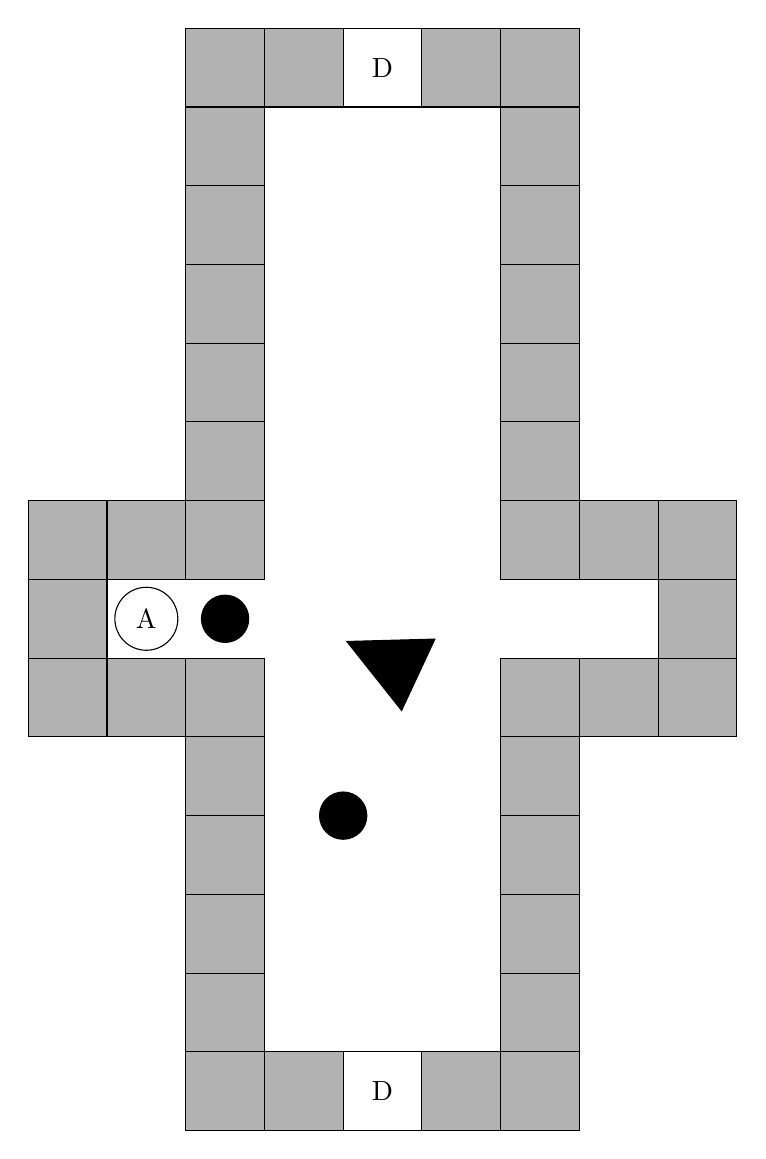
\begin{tikzpicture}[]

\newcommand{\wall}[2]{\filldraw[fill=black!30!white, draw=black] (#1,#2) rectangle (#1+1,#2+1);}
\newcommand{\area}[3]{\draw (#1,#2) rectangle (#1+1, #2+1) node[pos=.5] {#3};}
\newcommand{\door}[2]{\area{#1}{#2}{D};}
\newcommand{\player}[3]{\filldraw [fill=black, rotate around={#3:(#1,#2)}] (#1-0.5,#2-0.5) -- (#1,#2+0.5) -- (#1+0.5,#2-0.5) -- cycle;}
\newcommand{\enemy}[2]{\filldraw [fill=black] (#1,#2) circle(0.3) ;}

%top wall
\foreach \x in {0,...,1}
  \wall{\x}{0};
\door{2}{0}
\foreach \x in {3,...,4}
  \wall{\x}{0};

%bottom wall
\foreach \x in {3,...,4}
  \wall{\x}{13};
\door{2}{13}
\foreach \x in {0,...,1}
  \wall{\x}{13};

%left wall
\foreach \y in {1,...,5}
  \wall{0}{\y};
\foreach \y in {7,...,12}
  \wall{0}{\y};

%left indent
\foreach \y in {5,...,7}
  \wall{-2}{\y};
\foreach \x in {-1,...,-1}
  \wall{\x}{7};
\foreach \x in {-1,...,-1}
  \wall{\x}{5};

% right wall
\foreach \y in {1,...,5}
  \wall{4}{\y};
\foreach \y in {7,...,12}
  \wall{4}{\y};

%right indent
\foreach \y in {5,...,6}
  \wall{6}{\y};
\foreach \x in {5,...,6}
  \wall{\x}{7};
\foreach \x in {5,...,6}
  \wall{\x}{5};

\player{2.5}{6}{65}
\enemy{2}{4}
\enemy{0.5}{6.5}
\draw (-0.5,6.5) circle(0.4)  node {A};

\end{tikzpicture}
\end{document}